\documentclass{standalone}
\usepackage{amsmath, amsfonts, amsthm}
\usepackage[dvipsnames]{xcolor}
\usepackage{siunitx}
\usepackage{graphicx}
\usepackage{tikz}
\usepackage{circuitikz}
\usetikzlibrary{patterns}
\usepackage{scalerel}
\usepackage{pict2e}
\usepackage{tkz-euclide}
\usetikzlibrary{calc}
\usetikzlibrary{arrows.meta}
\usetikzlibrary{shadows}
\usetikzlibrary{external}
\usetikzlibrary{decorations.pathmorphing}
\usetikzlibrary{shapes.geometric}
\usetikzlibrary{arrows,shapes.gates.logic.US,shapes.gates.logic.IEC,calc}
\usepackage{pgfplots}
\pgfplotsset{compat=newest}
\usepgfplotslibrary{statistics}
\usepgfplotslibrary{fillbetween}

\begin{document}
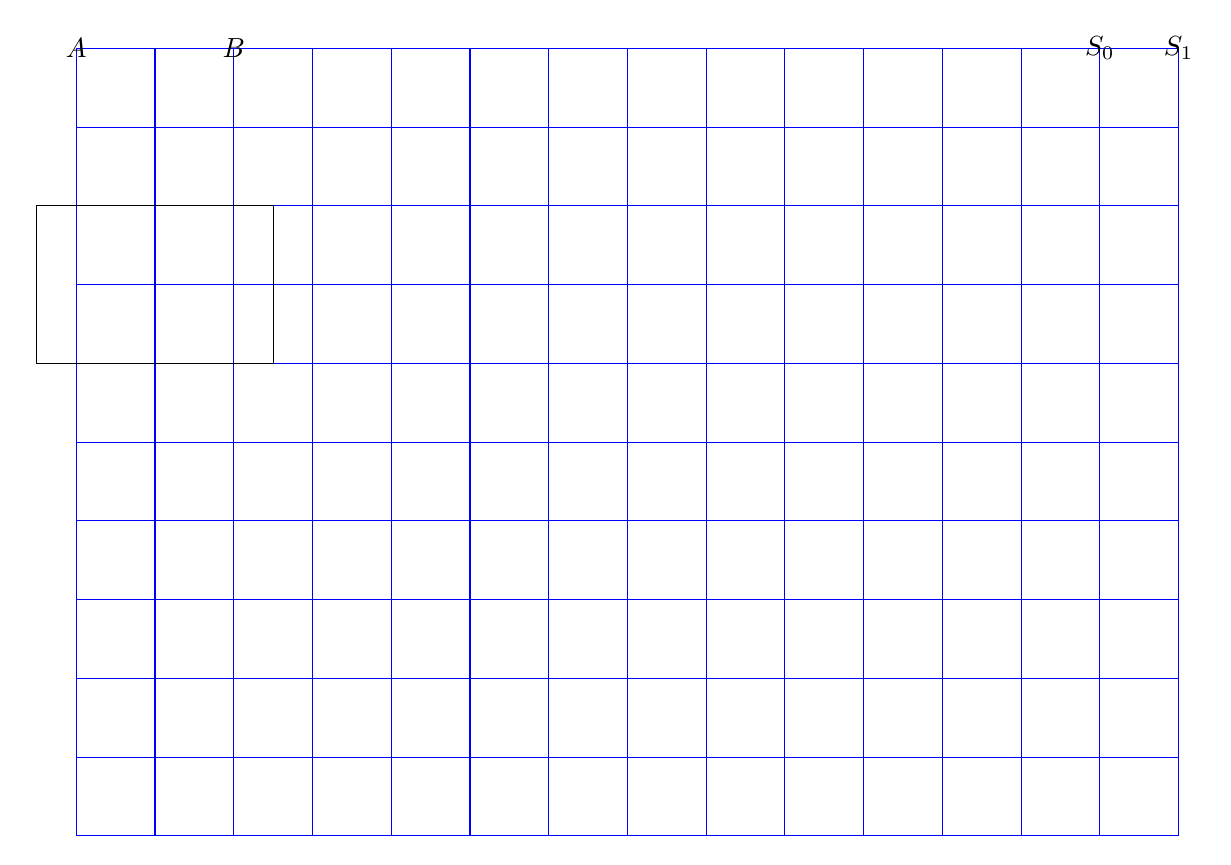
\begin{tikzpicture}
	%\draw [help lines, step=0.1, gray] (0,0) grid (10, -10);
	\draw [help lines, blue] (0,0) grid (14, -10);

	\node (A) at (0,0) {$A$};

	\node (B) [right of=A, shift={(1, 0)}] {$B$};

	\node (S0) [right of=B, shift={(10, 0)}] {$S_0$};
	\node (S1) [right of=S0] {$S_1$};

	\node (AND) [below of=A, shift={(-.5, -1)}] { };
	\draw [black, thin] (AND) rectangle ++(3, -2);  

	\end{tikzpicture}
\end{document}
